

\section{Background}
\label{sec:background}

In this section, we first present an example of commit change motivating our deep learning framework. We then briefly introduce background knowledge about Convolutional Neural Network (CNN) used to extract features in the commit change. 

\subsection{A Buggy Commit And Process Of Reviewing Commits}
\label{sec:examle}

\begin{figure}[t!]
\center
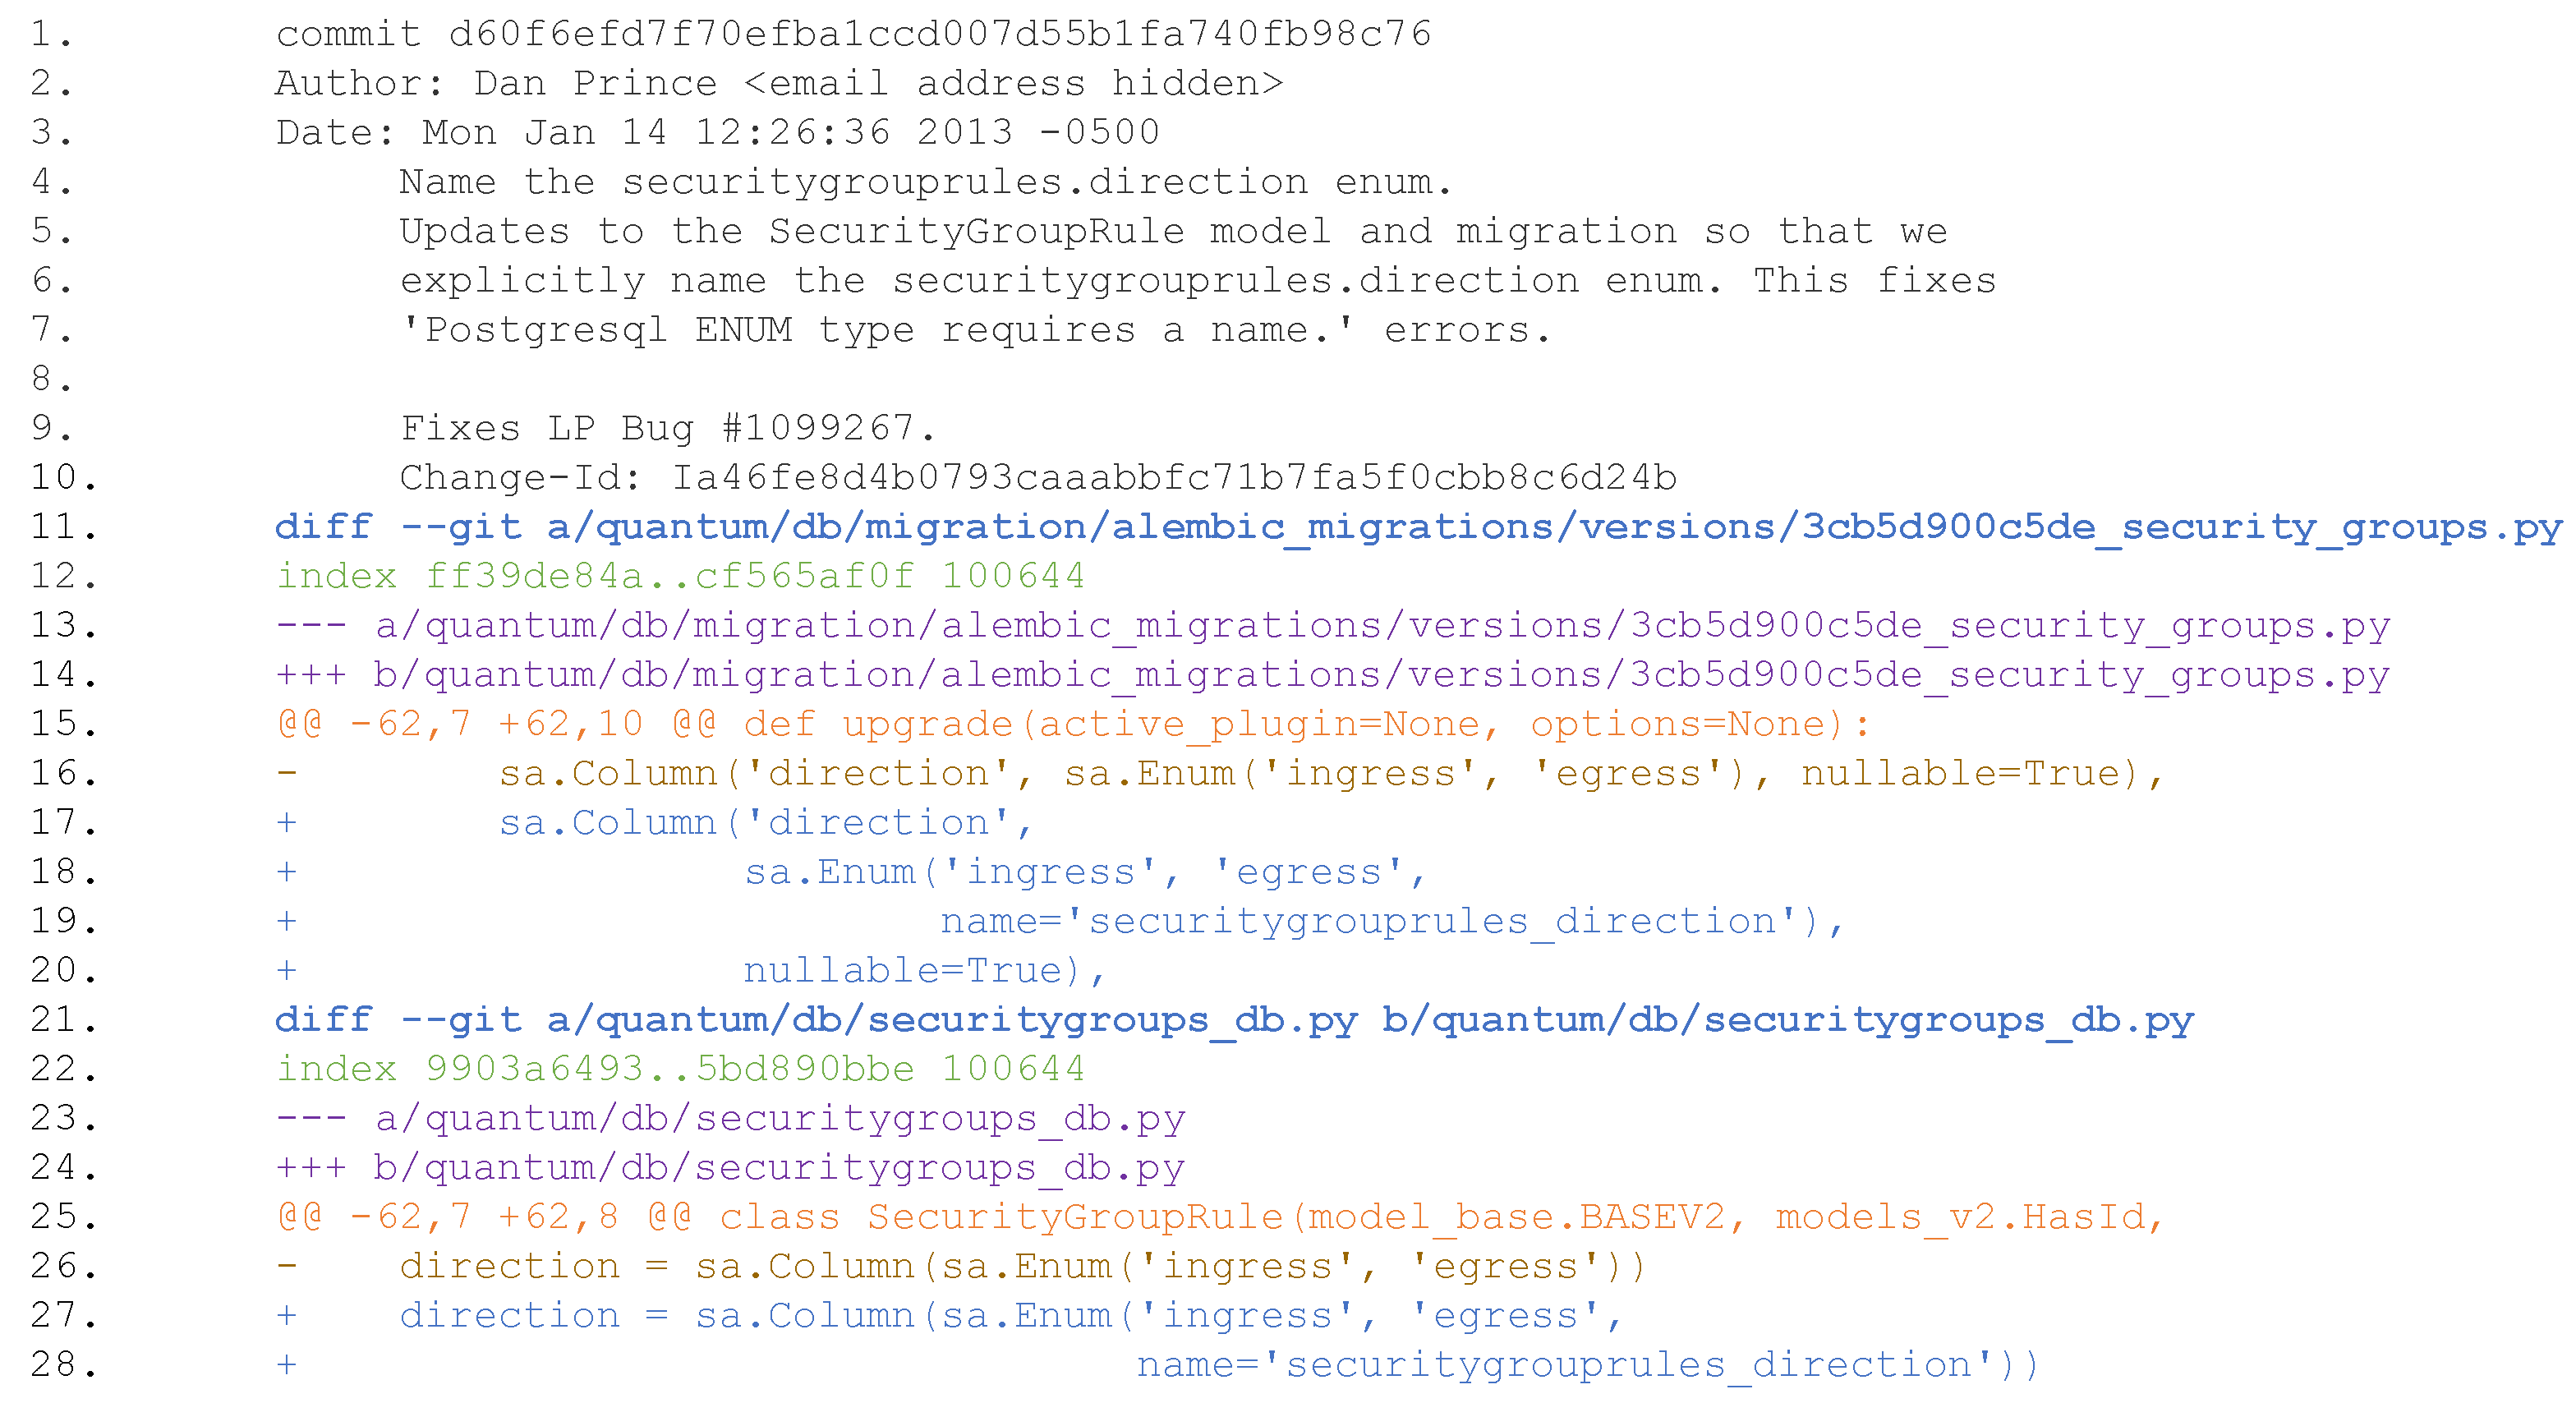
\includegraphics[scale=0.2]{figs/example.pdf}
\caption{An example of a buggy commit change in OPENSTACK.}
\label{fig:example}
\end{figure} 

Figure~\ref{fig:example} shows an example of a buggy commit in OPENSTACK. The buggy commit contains many pieces of information, i.e., a commit id (line 1), an author name (line 2), a commit date (line 3), a commit message (line 4-10) and a set of code changes (i.e., 11-28). A set of code changes includes changes of multiple files and each file includes a number of deleted and added lines representing the change. In the Figure~\ref{fig:example}, line 16 (starting with \texttt{-}) and lines 17-20 (starting with \texttt{+}) indicates the deleted and added lines of a change file (namely \texttt{3cb5d900c5de$\_$security$\_$groups.py}), respectively. The commit message also plays an important role as a good commit message can help maintainers to speed up the reviewing process and write a good release note.

To review a commit, QT and OPENSTACK use Gerrit~\footnote{https://code.google.com/p/gerrit/}, which is a code review tool for \texttt{git}-based software project. The process of reviewing code changes is as follows:
\begin{itemize}
    \item Upload change revision: An author of a code changes submits a new change to Gerrit and invites reviewers to comment it.
    \item Execute sanity tests: Sanity tests verify that the code changes are compliant with the coding style conventions before sending to the reviewers.
    \item Solicit peer feedback: The reviewers are asked to examine the code changes after it passes the sanity tests.
    \item Initiate integration request: Teams are allowed to verify the code changes before integrating it into \texttt{git} repositories.
    \item Execute integration tests: The integration testing system is run to ensure that the code changes that put in the \texttt{git} repositories is clean.
    \item Final integration: After passing the integration testing, Gerrit automatically commits the code changes into the \texttt{git} repositories.
\end{itemize}

On occasion,  we omit the code review process due to a rush to integrate critical code
changes. However, most code changes follow the code review process.

% Previous works mainly depend on a set of manually defined features extracted from code changes~\cite{Yang:2015:DLJ, mcintosh2018fix}, however, the set of manual code features might overlook some helpful features to identify a buggy commit. Moreover, past studies also ignore the commit message. Thus, potentially rich source of information has not been tapped yet. 

\subsection{Convolutional Neural Network}
\label{sec:background_cnn}

\begin{figure*}[t!]
	\center
	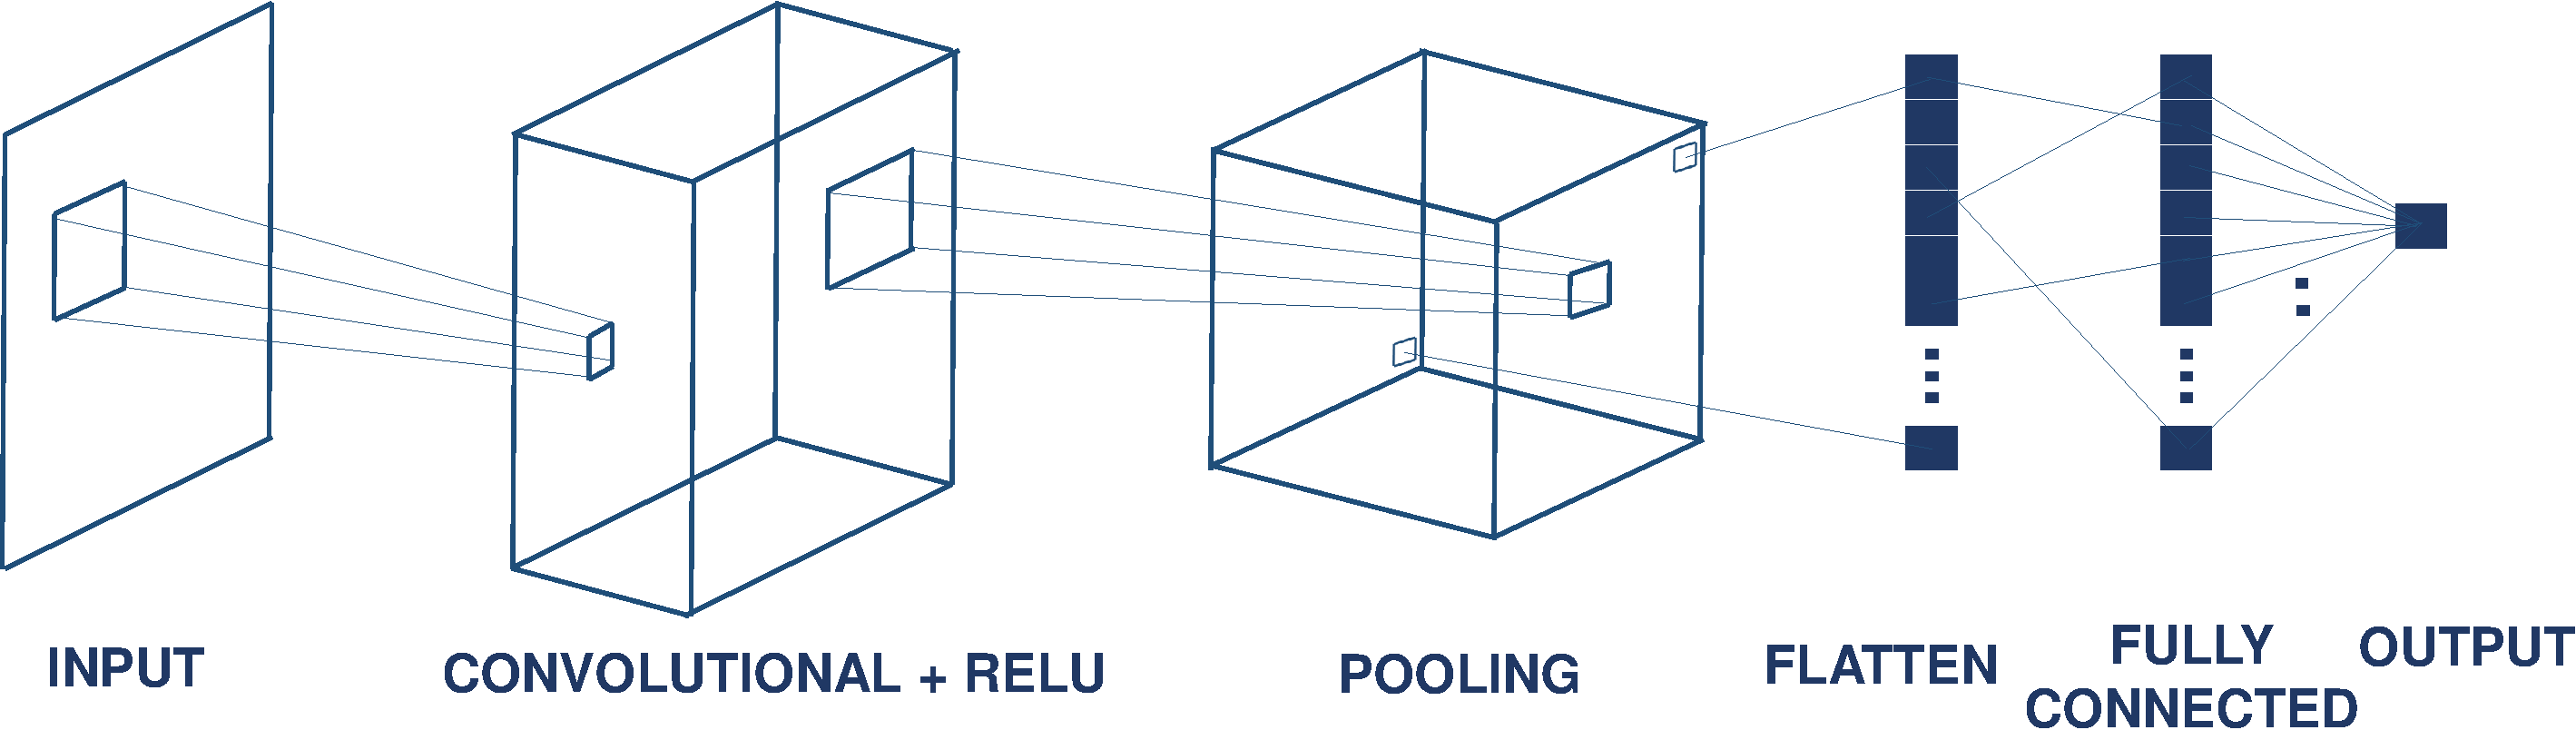
\includegraphics[scale=0.3]{figs/cnn.pdf}
	\caption{A simple convolutional neural network architecture.}
	\label{fig:cnn}
\end{figure*}

\begin{figure*}[t!]
	\center
	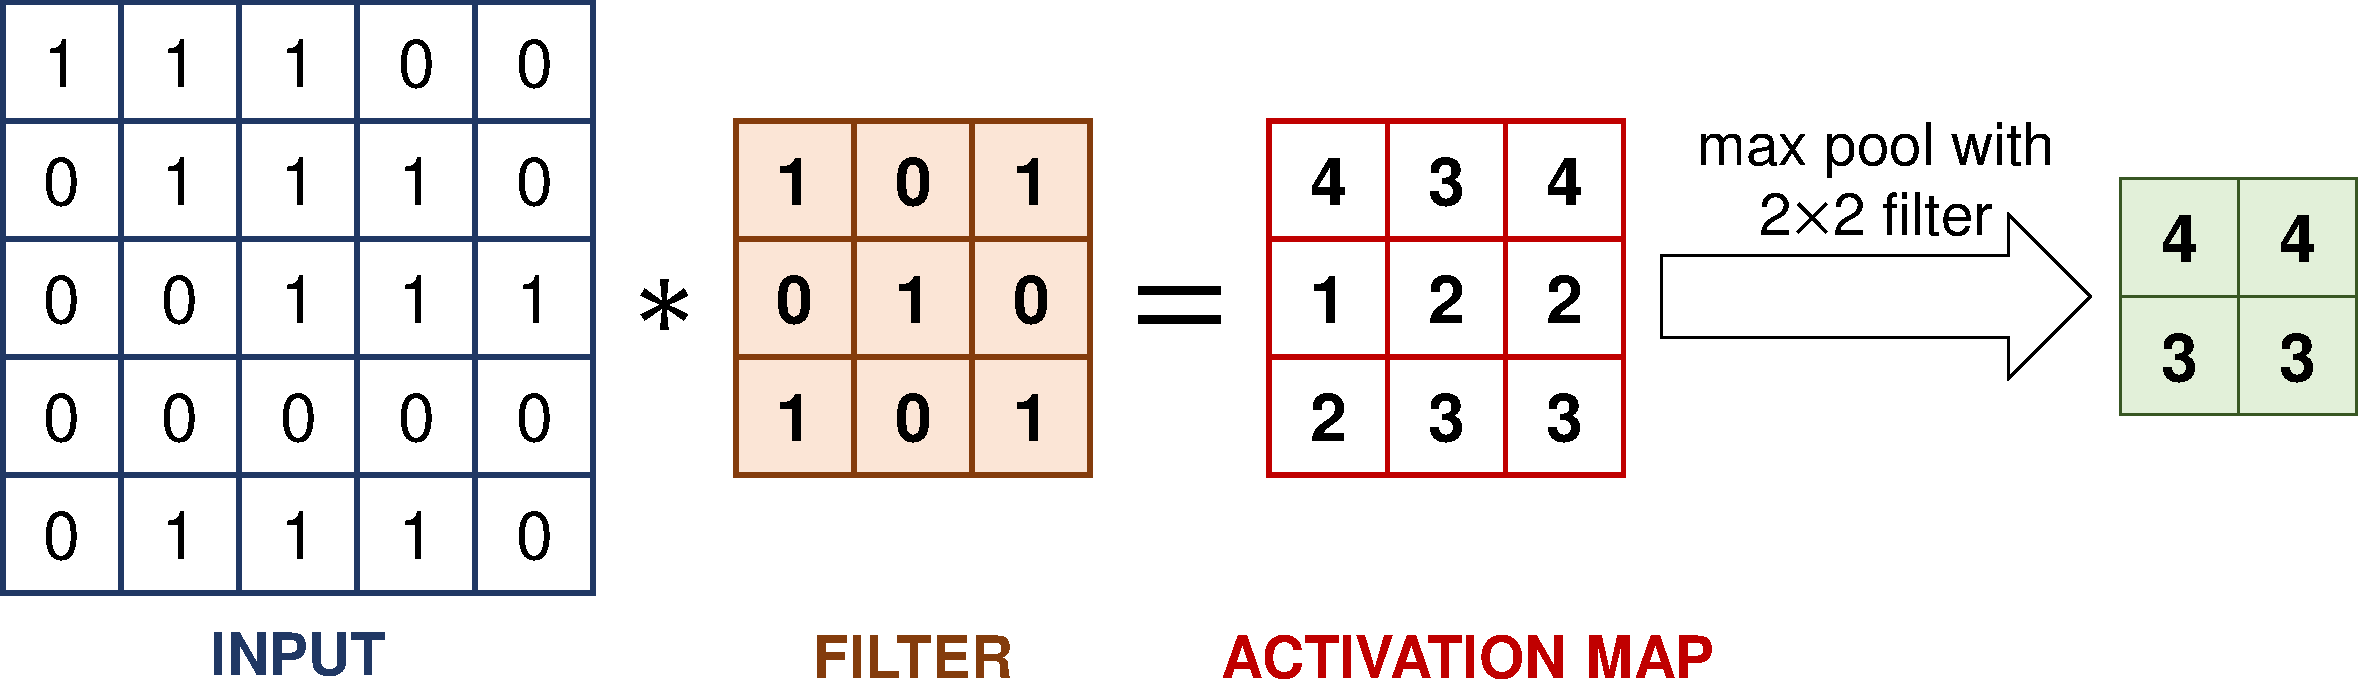
\includegraphics[scale=0.28]{figs/filter_pooling.pdf}
	\caption{An example of a convolutional layer and pooling layer in CNN.}
	\label{fig:filter}
\end{figure*}

One of the most powerful forms of deep learning neural networks is the Convolutional Neural Network (CNN)~\cite{lecun2015deep}. CNNs are widely used in many problems (i.e., image pattern recognition, natural language processing, information retrieval, etc.) and have been achieved significant results~\cite{karpathy2014large, lawrence1997face, krizhevsky2012imagenet}. Like traditional deep learning networks, CNNs receive an input and perform a product operation followed by a nonlinear function. The last layer is the output layer containing objective functions~\cite{zhao2017loss} associated with the labels of the input.

Figure~\ref{fig:cnn} illustrates a simple CNN for classification task. The simple CNN includes an input layer, a convolutional layer, followed by the rectified linear unit (RELU) which is a nonlinear activation function, a pooling layer, a fully-connected layer, and an output layer. We briefly explain these layers in the following paragraphs. 

The input layer takes an input as 2-dimensional array or 3-dimensional array and passes it through a of convolution layers.

The convolutional layer plays a vital role in CNN and it takes advantage of the use of learnable filters. These filters are small in spatial dimensionality, but they are applied along the entirety of the depth of the input data. For example, given an input data $\textbf{I} \in \mathbb{R}^{\text{H} \times \text{W} \times \text{D}}$ and a filter $\textbf{K} \in \mathbb{R}^{\text{h} \times \text{w} \times \text{D}}$, we produce a new activation map $\textbf{A} \in \mathbb{R}^{(\text{H} - \text{h}) \times (\text{W} - \text{w}) \times 1}$. The RELU is then applied to each value of the activation map as follows:
\begin{equation}
\label{eq:relu}
f(x) = max(0, x)   
\end{equation}

The pooling layer aims to reduce the dimensionality of the activation map, the number of parameters, and the computational helping to control overfitting problem~\cite{tolias2015particular}. The pooling layer spreads along the activation map and scales its dimensionality. There are three different types of pooling layers:
\begin{itemize}
	\item Max pooling takes the largest element from each region of the activation map.
	\item Average pooling constructs the average value from each region of the activation map.
	\item Sum pooling sums all the elements from each region of the activation map. 
\end{itemize}
In practice, max pooling often achieves a better performance compared to the other two pooling techniques~\cite{zeiler2013stochastic}. Figure~\ref{fig:filter} presents a visual representation of a convolutional layer and pooling layer in CNN. Given an input 5$\times$5 and a filter 3$\times$3, we output a new activation map 3$\times$3. A max pooling layer with a filter 2$\times$2 is then applied to produce a new output. 

The output of pooling layer is flatten and directly passed to a fully connected layer. The fully connected layer is passed to an output layer to calculate an objective function (or a loss function)~\cite{zhao2017loss}. The objective function normally is optimized using a stochastic gradient descent (SGD)~\cite{bottou2010large}. This is an analogous way with traditional neural networks~\cite{huang1988neural}.



